% !TeX program = xelatex
\documentclass[10pt,a4paper]{ctexart} % 设置文章类型，正文字号与纸张大小

% 页面与正文常用宏包
\usepackage[margin=2cm]{geometry} % 设置页面四周页边距
\usepackage{graphicx}             % 插入图片
\usepackage{amsmath}              % 提供cases、aligned等数学公式环境
\usepackage{amssymb}              % 提供\therefore等扩展数学符号
\usepackage{booktabs}             % 提供\toprule、\midrule、\bottomrule三线表命令
\usepackage{float}                % 提供[H]固定图片、表格位置
\usepackage{subcaption}           % 提供subfigure子图环境及子图标题
\usepackage{wrapfig}              % 提供wrapfigure图文环绕环境
\usepackage{fancyhdr}             % 自定义页眉和页脚
\usepackage{hyperref}             % 生成超链接

% 页眉页脚
\pagestyle{fancy}                  % 启用fancyhdr定义的页面样式
\fancyhf{}                         % 清空默认页眉和页脚
\fancyfoot[C]{\thepage}            % 在页脚中央显示页码
\renewcommand{\headrulewidth}{0pt} % 隐藏页眉横线
\renewcommand{\footrulewidth}{0pt} % 隐藏页脚横线

% 超链接
\hypersetup{
  colorlinks=true,                % 使用彩色文字链接，而非带边框的链接
  linkcolor=red,                 % 目录、公式及图表交叉引用的颜色
  filecolor=cyan,                 % 本地文件链接的颜色
  urlcolor=blue,                  % 网址链接的颜色
  pdftitle={光电效应测定普朗克常量报告},     % 写入PDF文档属性的标题
  bookmarksnumbered=true          % PDF书签显示章节编号
}

% 定义字号命令
\newcommand{\chuhao}{\fontsize{42pt}{63pt}\selectfont}
\newcommand{\xiaochu}{\fontsize{36pt}{54pt}\selectfont}
\newcommand{\yihao}{\fontsize{26pt}{39pt}\selectfont}
\newcommand{\xiaoyi}{\fontsize{24pt}{36pt}\selectfont}
\newcommand{\erhao}{\fontsize{22pt}{33pt}\selectfont}
\newcommand{\xiaoer}{\fontsize{18pt}{27pt}\selectfont}
\newcommand{\sanhao}{\fontsize{16pt}{24pt}\selectfont}
\newcommand{\xiaosan}{\fontsize{15pt}{22.5pt}\selectfont}
\newcommand{\sihao}{\fontsize{14pt}{21pt}\selectfont}
\newcommand{\xiaosi}{\fontsize{12pt}{18pt}\selectfont}
\newcommand{\wuhao}{\fontsize{10.5pt}{15.75pt}\selectfont}
\newcommand{\xiaowu}{\fontsize{9pt}{13.5pt}\selectfont}

% 章节格式
\ctexset{
  section={
    format={\CJKfontspec[AutoFakeBold=2.5]{KaiTi}\sanhao\bfseries}, % 一级标题使用三号加粗楷体
    name={,、},                                                    % 在中文章节序号后添加顿号
    number=\chinese{section},                                      % 一级标题编号使用“一、二、三”形式
    aftername={}                                                   % 取消编号与标题文字之间的空格
  },
  subsection={
    format={\CJKfontspec[AutoFakeBold=2.5]{KaiTi}\sihao\bfseries}, % 二级标题使用四号加粗楷体                                               
  },
  subsubsection={
    format={\CJKfontspec[AutoFakeBold=2.5]{KaiTi}\xiaosi\bfseries}, % 三级标题使用小四加粗楷体
  }
}
\begin{document}

% 封面
\thispagestyle{fancy} % 封面保留底部居中的页码
\fancyfoot[C]{\thepage}
\begin{center}
  \CJKfontspec[AutoFakeBold=2.5]{KaiTi}\bfseries % 封面中文使用楷体并人工加粗，西文同时加粗
  \vspace{0.8cm}
  
\includegraphics[width=8.2cm]{figures/head.png}

  \vspace{0.2cm}
  \xiaochu 
    物理实验报告

  \vspace{3.5cm}
  \begin{minipage}{10.0cm}
    \sanhao
    \makebox[2.6cm][l]{实验名称：}
    \underline{\makebox[7.0cm][c]{光电效应测定普朗克常量}}\par\vspace{12pt}

    \makebox[2.6cm][l]{实验桌号：}
    \underline{\makebox[7.0cm][c]{13}}\par\vspace{12pt}

    \makebox[2.6cm][l]{指导教师：}
    \underline{\makebox[7.0cm][c]{史明}}
  \end{minipage}

  \vspace{3.5cm}
  \begin{minipage}{10.0cm}
    \sihao
    \makebox[1.4cm][l]{班级：}
    \underline{\makebox[8.0cm][c]{信工2503}}\par\vspace{10pt}

    \makebox[1.4cm][l]{姓名：}
    \underline{\makebox[8.0cm][c]{陈源}}\par\vspace{10pt}

    \makebox[1.4cm][l]{学号：}
    \underline{\makebox[8.0cm][c]{3250103617}}
  \end{minipage}

  \vspace{2.0cm}
  \sihao
    实验日期：
    \underline{\makebox[0.7cm][c]{2026}}年
    \underline{\makebox[0.7cm][c]{11}}月
    \underline{\makebox[0.7cm][c]{18}}日
    星期\underline{\makebox[0.7cm][c]{三}}上午

  \vspace{0.7cm}
  \sihao 
    浙江大学物理实验教学中心
\end{center}

\newpage
\xiaosi\songti\mdseries % 后续正文统一使用小四不加粗的宋体

\section{预习报告（10分）}

  \subsection{实验综述（5分）}
  
    \subsubsection{普朗克常数的多种测定方法}
    常用方法有黑体辐射法、光电效应法、X射线法、康普顿散射法、约瑟夫森效应法、量子霍尔效应法和力学天平法。

    本实验采用光电效应法，普朗克常数的参考值约为 \mbox{$h = 6.626\times 10^{-34}\,\mathrm{J\cdot s}$}。

    \subsubsection{实验原理}
    \begin{figure} [H]
      \centering
      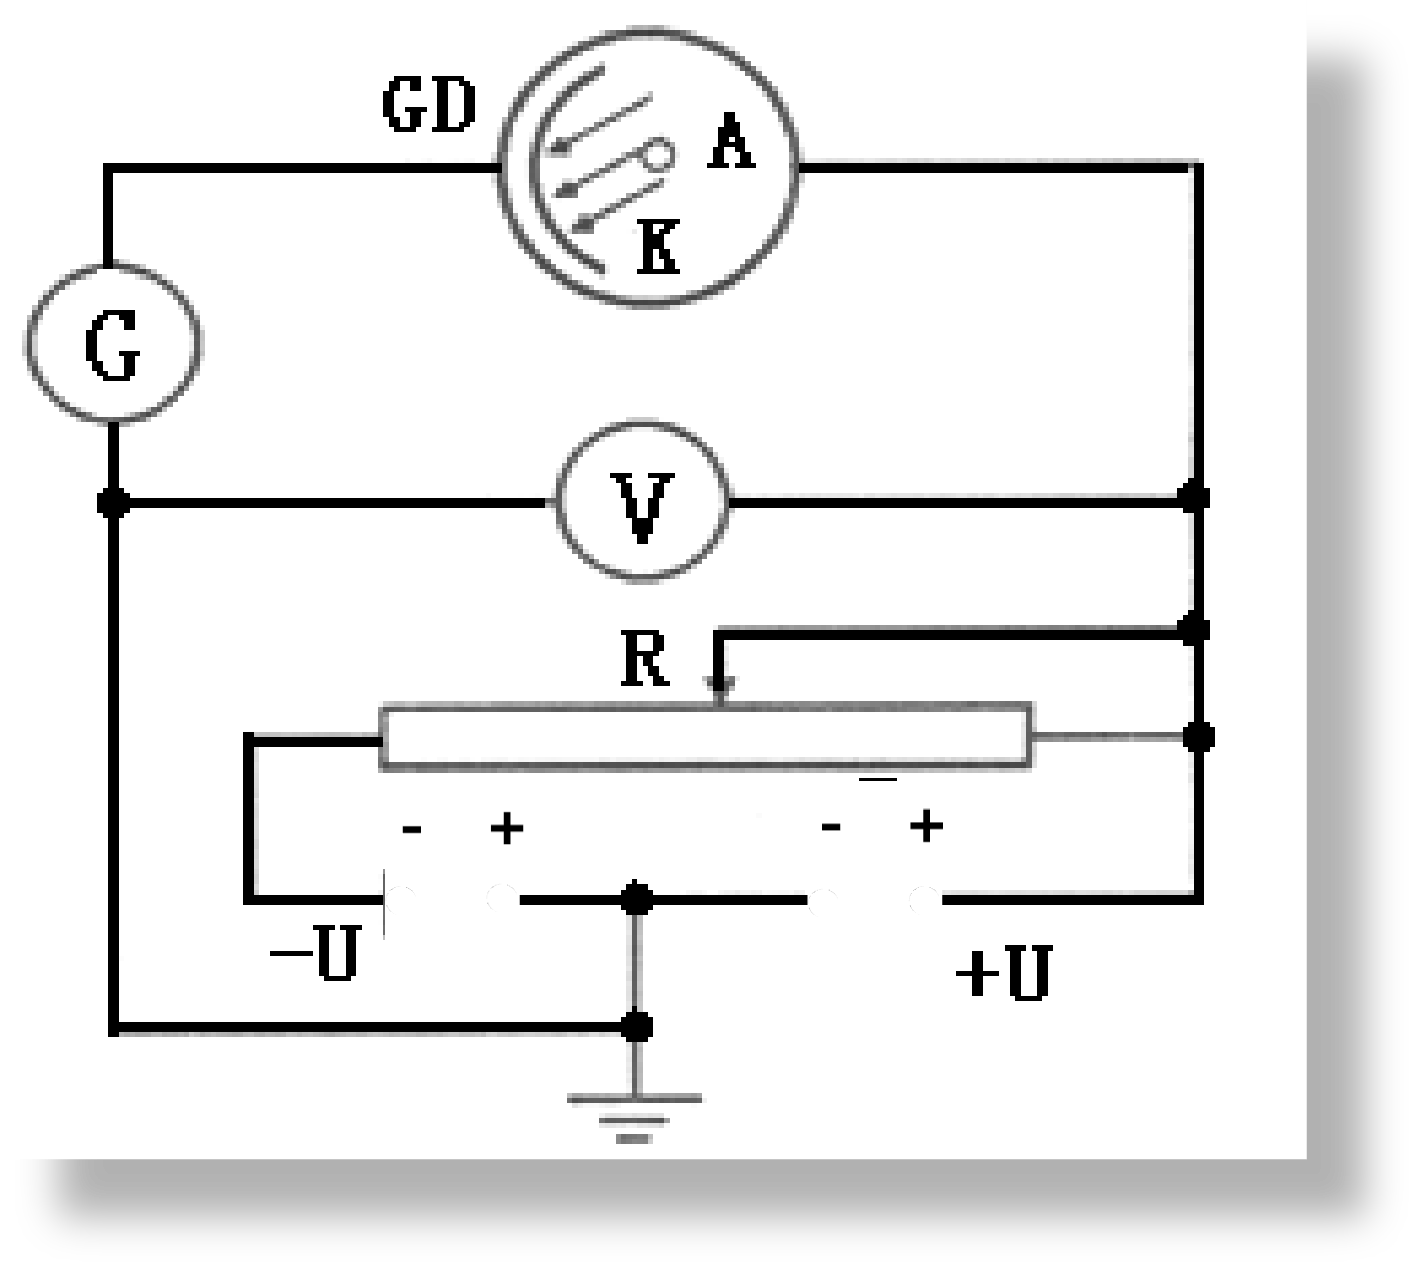
\includegraphics[width=0.35\textwidth]{figures/图1.png}
      \caption{光电效应实验示意图}
    \end{figure}

    图中，GD为光电管，K、A分别为阴极和阳极，G为微检流计，V为电压表，$\pm U$为电源，R为滑线变阻器。
    光照阴极使电子吸收光子能量后逸出，形成光电流；改变外加电压可测得伏安特性。

    光电效应具有以下规律：
    \begin{itemize}
      \item 光电子最大初动能随光频率线性变化，与光强无关；
      \item 光频率低于截止频率时，不产生光电子；
      \item 频率一定时，饱和光电流与光强成正比；
      \item 光电子发射具有瞬时性。
    \end{itemize}

    爱因斯坦光电效应方程为
    \[
    h\nu = \frac{1}{2}mv_{\max}^2 + W
    \]
    
    其中 $W$ 为阴极材料的逸出功。施加反向电压，使光电流恰好降为零时，其电压大小称为截止电压 $U_a$，满足 $eU_a=\frac{1}{2}mv_{\max}^2$。

    \begin{figure}[H]
      \centering
      \begin{minipage}{0.4\textwidth}
        \centering
        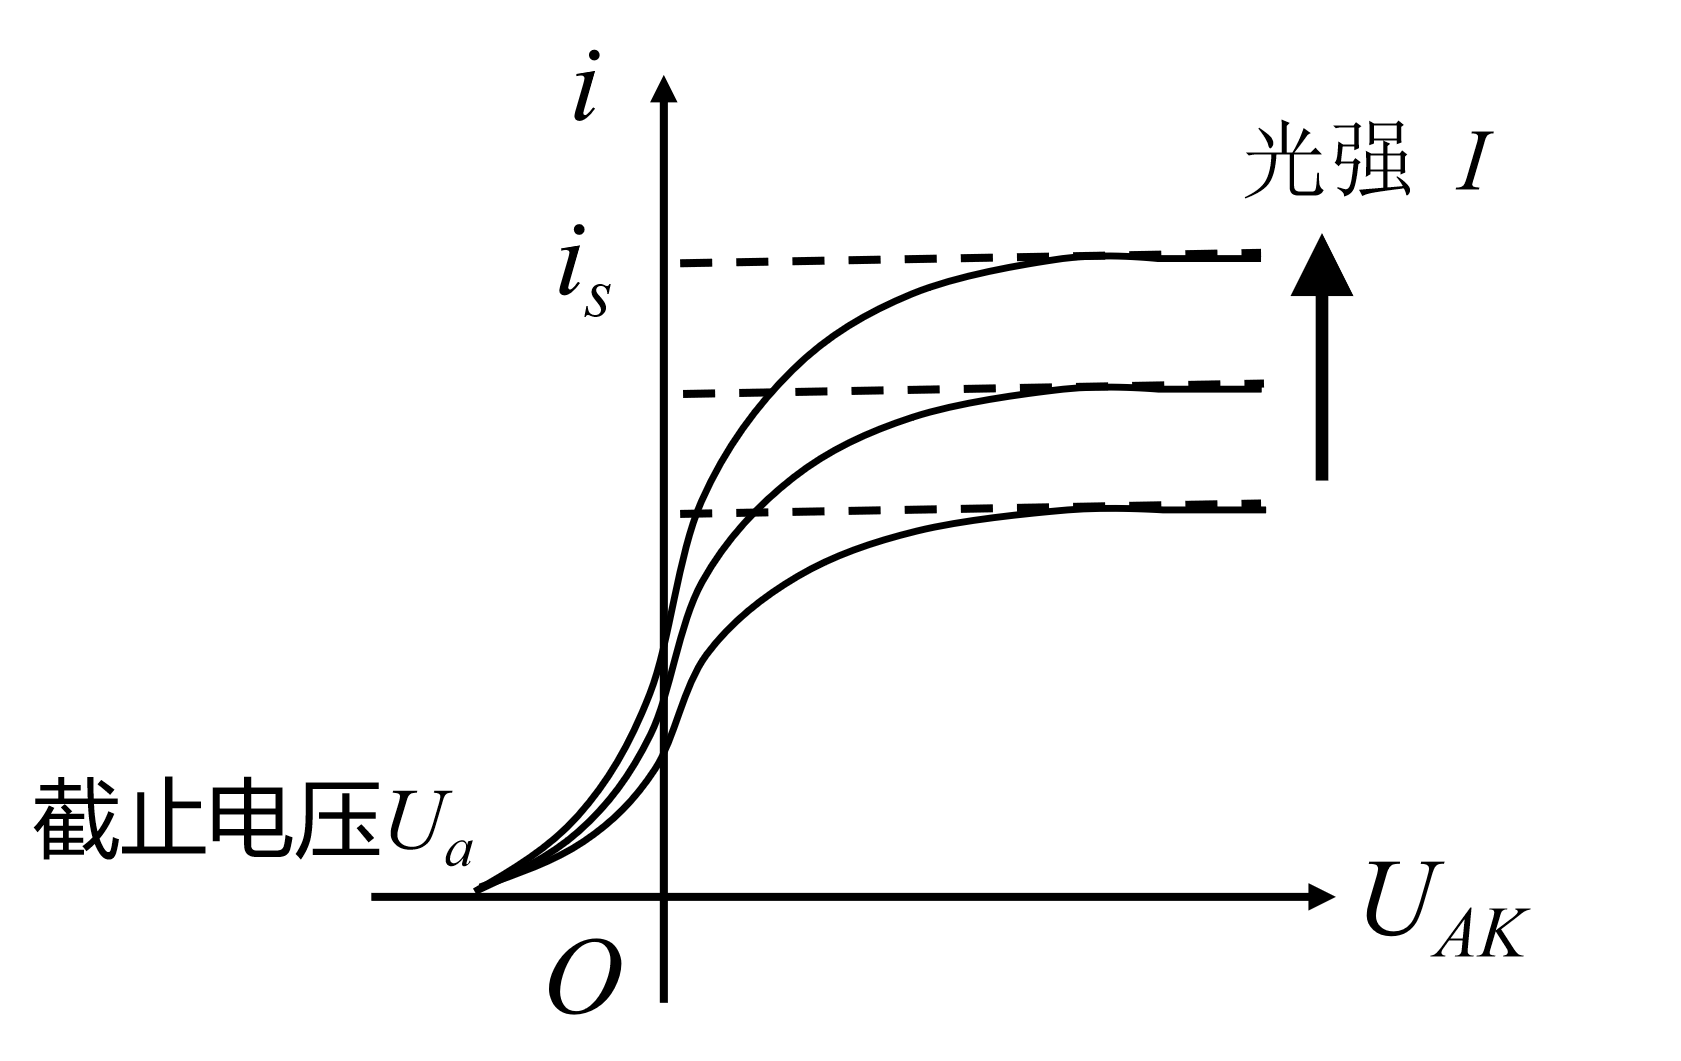
\includegraphics[width=\linewidth]{figures/图2.png}
        \caption{截止电压，饱和电流与光强}
      \end{minipage}
      \hfill
      \begin{minipage}{0.3\textwidth}
        \centering
        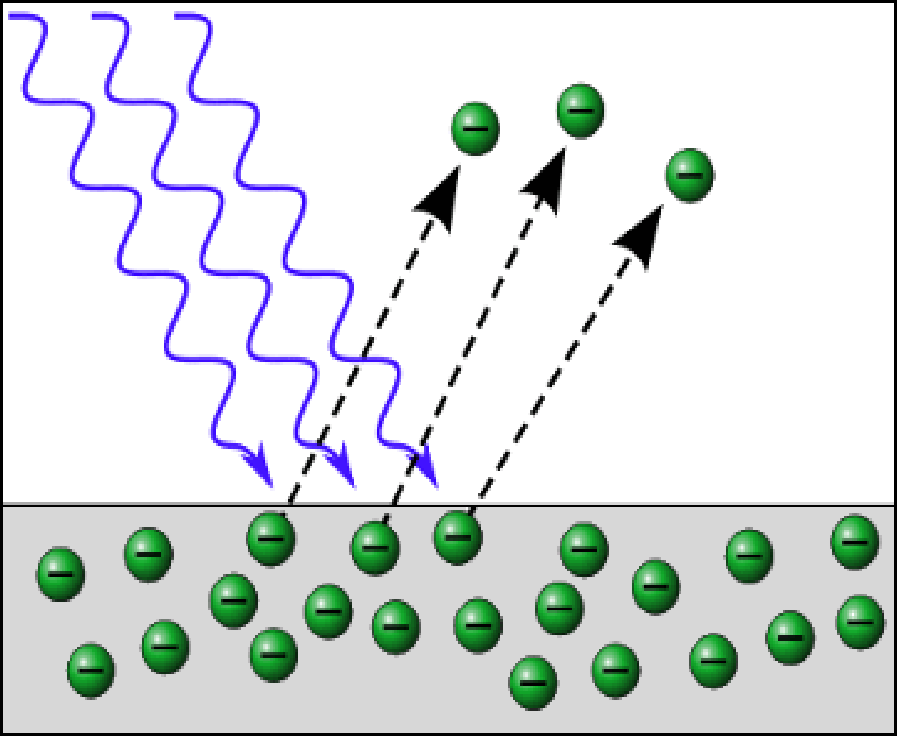
\includegraphics[width=\linewidth]{figures/图3.png}
        \caption{爱因斯坦光电效应方程}
      \end{minipage}
    \end{figure}

    \begin{wrapfigure}{r}{0.4\textwidth}
      \centering
      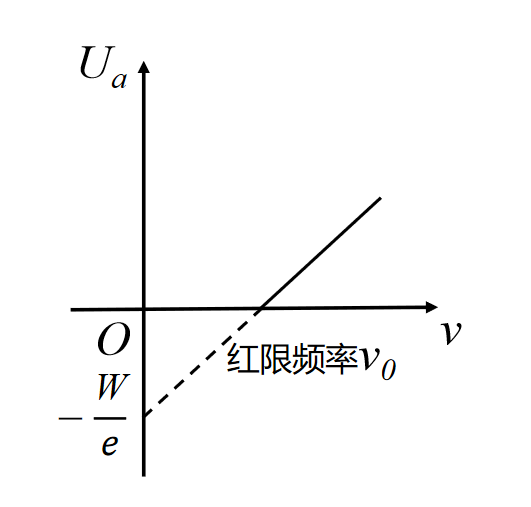
\includegraphics[width=\linewidth]{figures/图4.png}
      \caption{截止电压与频率的关系}
    \end{wrapfigure}

    由光电效应方程可得
    \[
    U_a = \frac{h}{e}\nu - \frac{W}{e},
    \qquad \nu_0 = \frac{W}{h}
    \]
    
    当 $\nu<\nu_0$ 时不发生光电效应；当 $\nu\geq\nu_0$ 时，截止电压与频率呈线性关系。
    测量不同频率下的截止电压并作线性拟合，由斜率 $k=h/e$ 求得 $h=ek$，由截距可求逸出功 $W$。

    \subsubsection{实验内容}
    \begin{enumerate}
      \item 使用不同滤光片，测量截止电压
      \item 使用不同滤光片，测量在单色光照射下的光电效应伏安特性曲线
      \item 在单色光照射下，探究光电管饱和光电流和光源距离的关系
      \item 在单色光照射下，探究光电管饱和光电流和光阑孔径大小的关系
    \end{enumerate} 

  \subsection{实验重点（3分）}
  \begin{enumerate}
    \item 理解光电效应方程和光量子概念
    \item 掌握光电效应实验方法并验证实验现象
    \item 测定普朗克常数
  \end{enumerate}

  \subsection{实验难点（2分）}
  \begin{enumerate}
    \item 准确判断光电流零点，测量各频率下的截止电压；
    \item 减小暗电流、接触电势及读数波动的影响；
    \item 对截止电压与频率作线性拟合，计算普朗克常量并分析误差。
  \end{enumerate}

\section{实验操作与原始数据（50分）}
\begin{figure}[H]
  \centering
  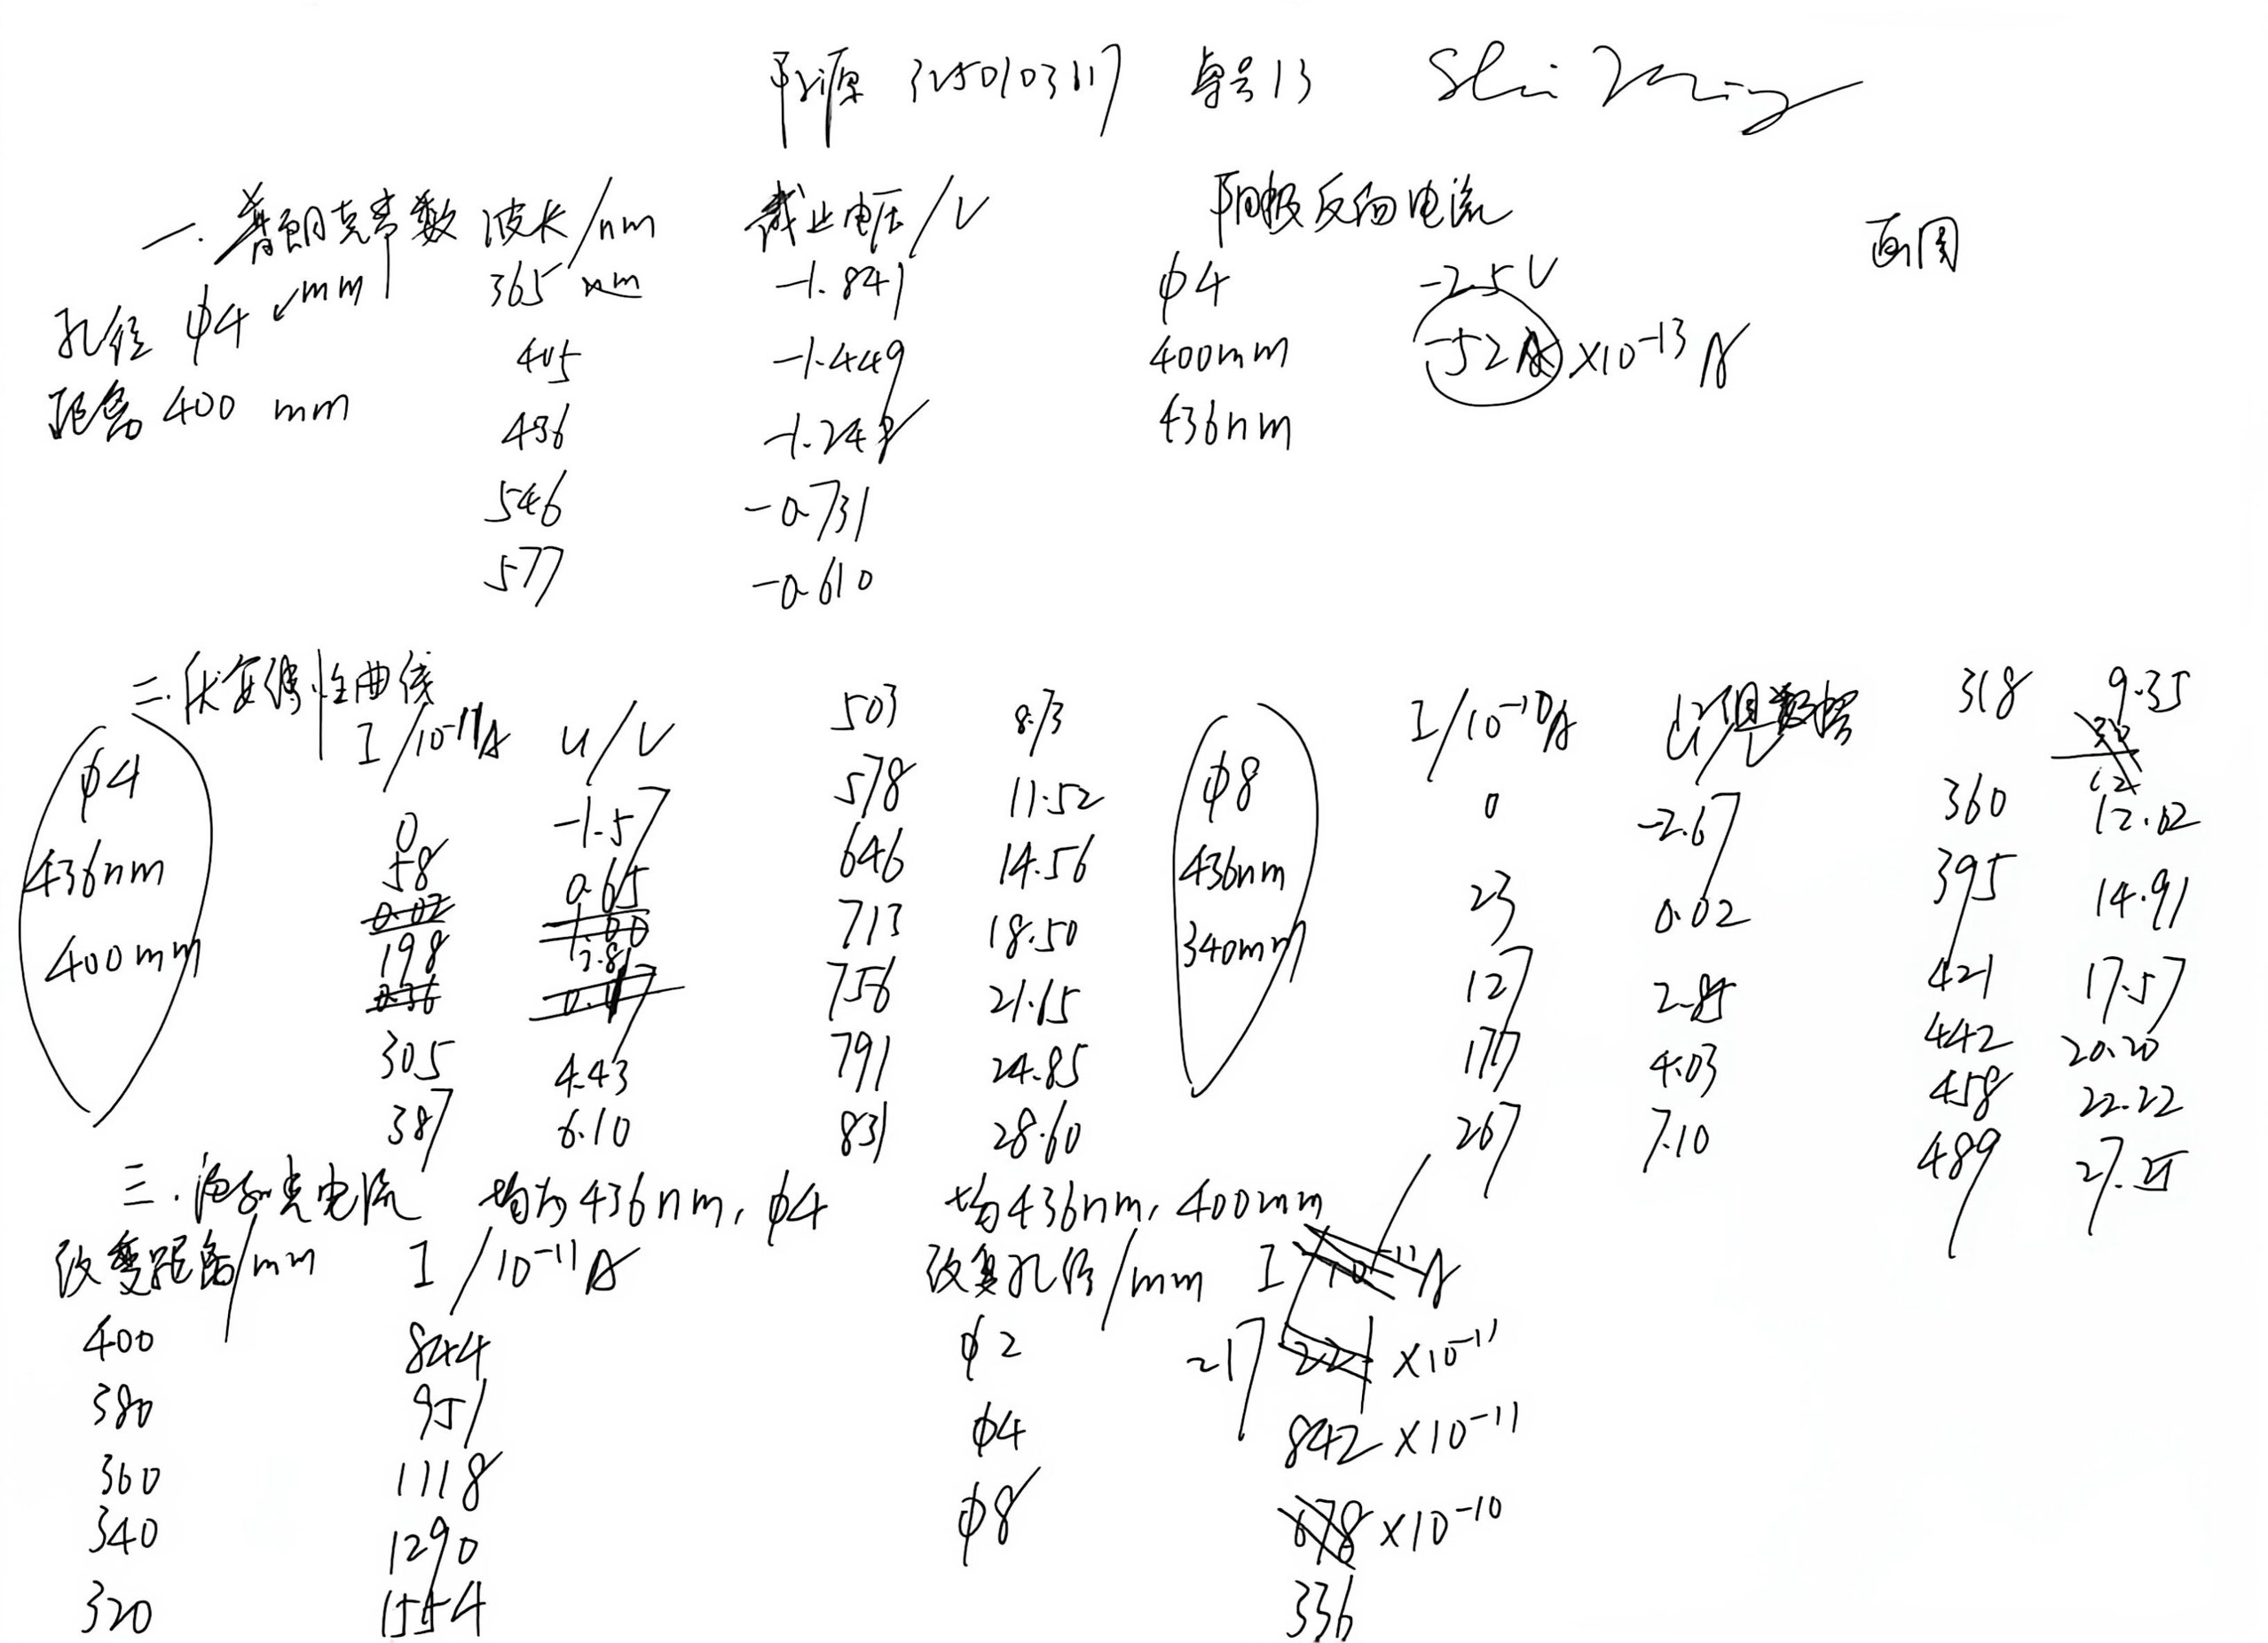
\includegraphics[width=0.75\textwidth]{figures/图5.png}
  \caption{实验原始数据}
\end{figure}

\section{结果与分析（30分）}

  \subsection{数据处理与结果（20分）}
  本次实验分为三个小实验：
  \begin{enumerate}
    \item 使用不同滤光片，测量截止电压，拟合曲线测定普朗克常量。
    \item 固定单色光波长，改变光阑孔径和光源距离，测量光电效应伏安特性曲线。
    \item 在单色光照射下，分别探究光电管饱和光电流，与光源距离和光阑孔径大小的关系。
  \end{enumerate}

  在这三个实验前，先测量一组阳极反向电流（滤光片波长：$436\,\mathrm{nm}$，光阑孔径$4\,\mathrm{mm}$，光源距离$40\,\mathrm{cm}$）。
  测得阳极反向电流为$-52\times10^{-13}\,\mathrm{A}$，负号表示其方向与正向光电流相反。
  该电流主要由阳极受散射光照射后发射光电子产生。

  \subsubsection{普朗克常量的测定}
    实验测定数据如下：

    \begin{table}[H]
      \centering
      \caption{普朗克常量的测定（光阑孔径：$4\,\mathrm{mm}$，光源距离：$40\,\mathrm{cm}$）}
      \begin{tabular}{cccccc}
        \toprule
        滤光片波长$\lambda$（nm） & 365 & 405 & 436 & 546 & 577 \\
        \midrule
        截止电压$U_a$（V） & -1.841 & -1.449 & -1.248 & -0.731 & -0.610 \\
        频率$\nu$（$10^{14}\,\mathrm{Hz}$） & 8.213 & 7.402 & 6.876 & 5.491 & 5.196 \\
        \bottomrule
      \end{tabular}
    \end{table}

    由$\nu=c/\lambda$计算各单色光的频率。表1中记录的是仪器测量的负电压，作图及计算时应该取其绝对值$U=|U_a|$，
    绘制$U$--$\nu$关系并进行最小二乘直线拟合，如图6所示。

    \begin{figure}[H]
      \centering
      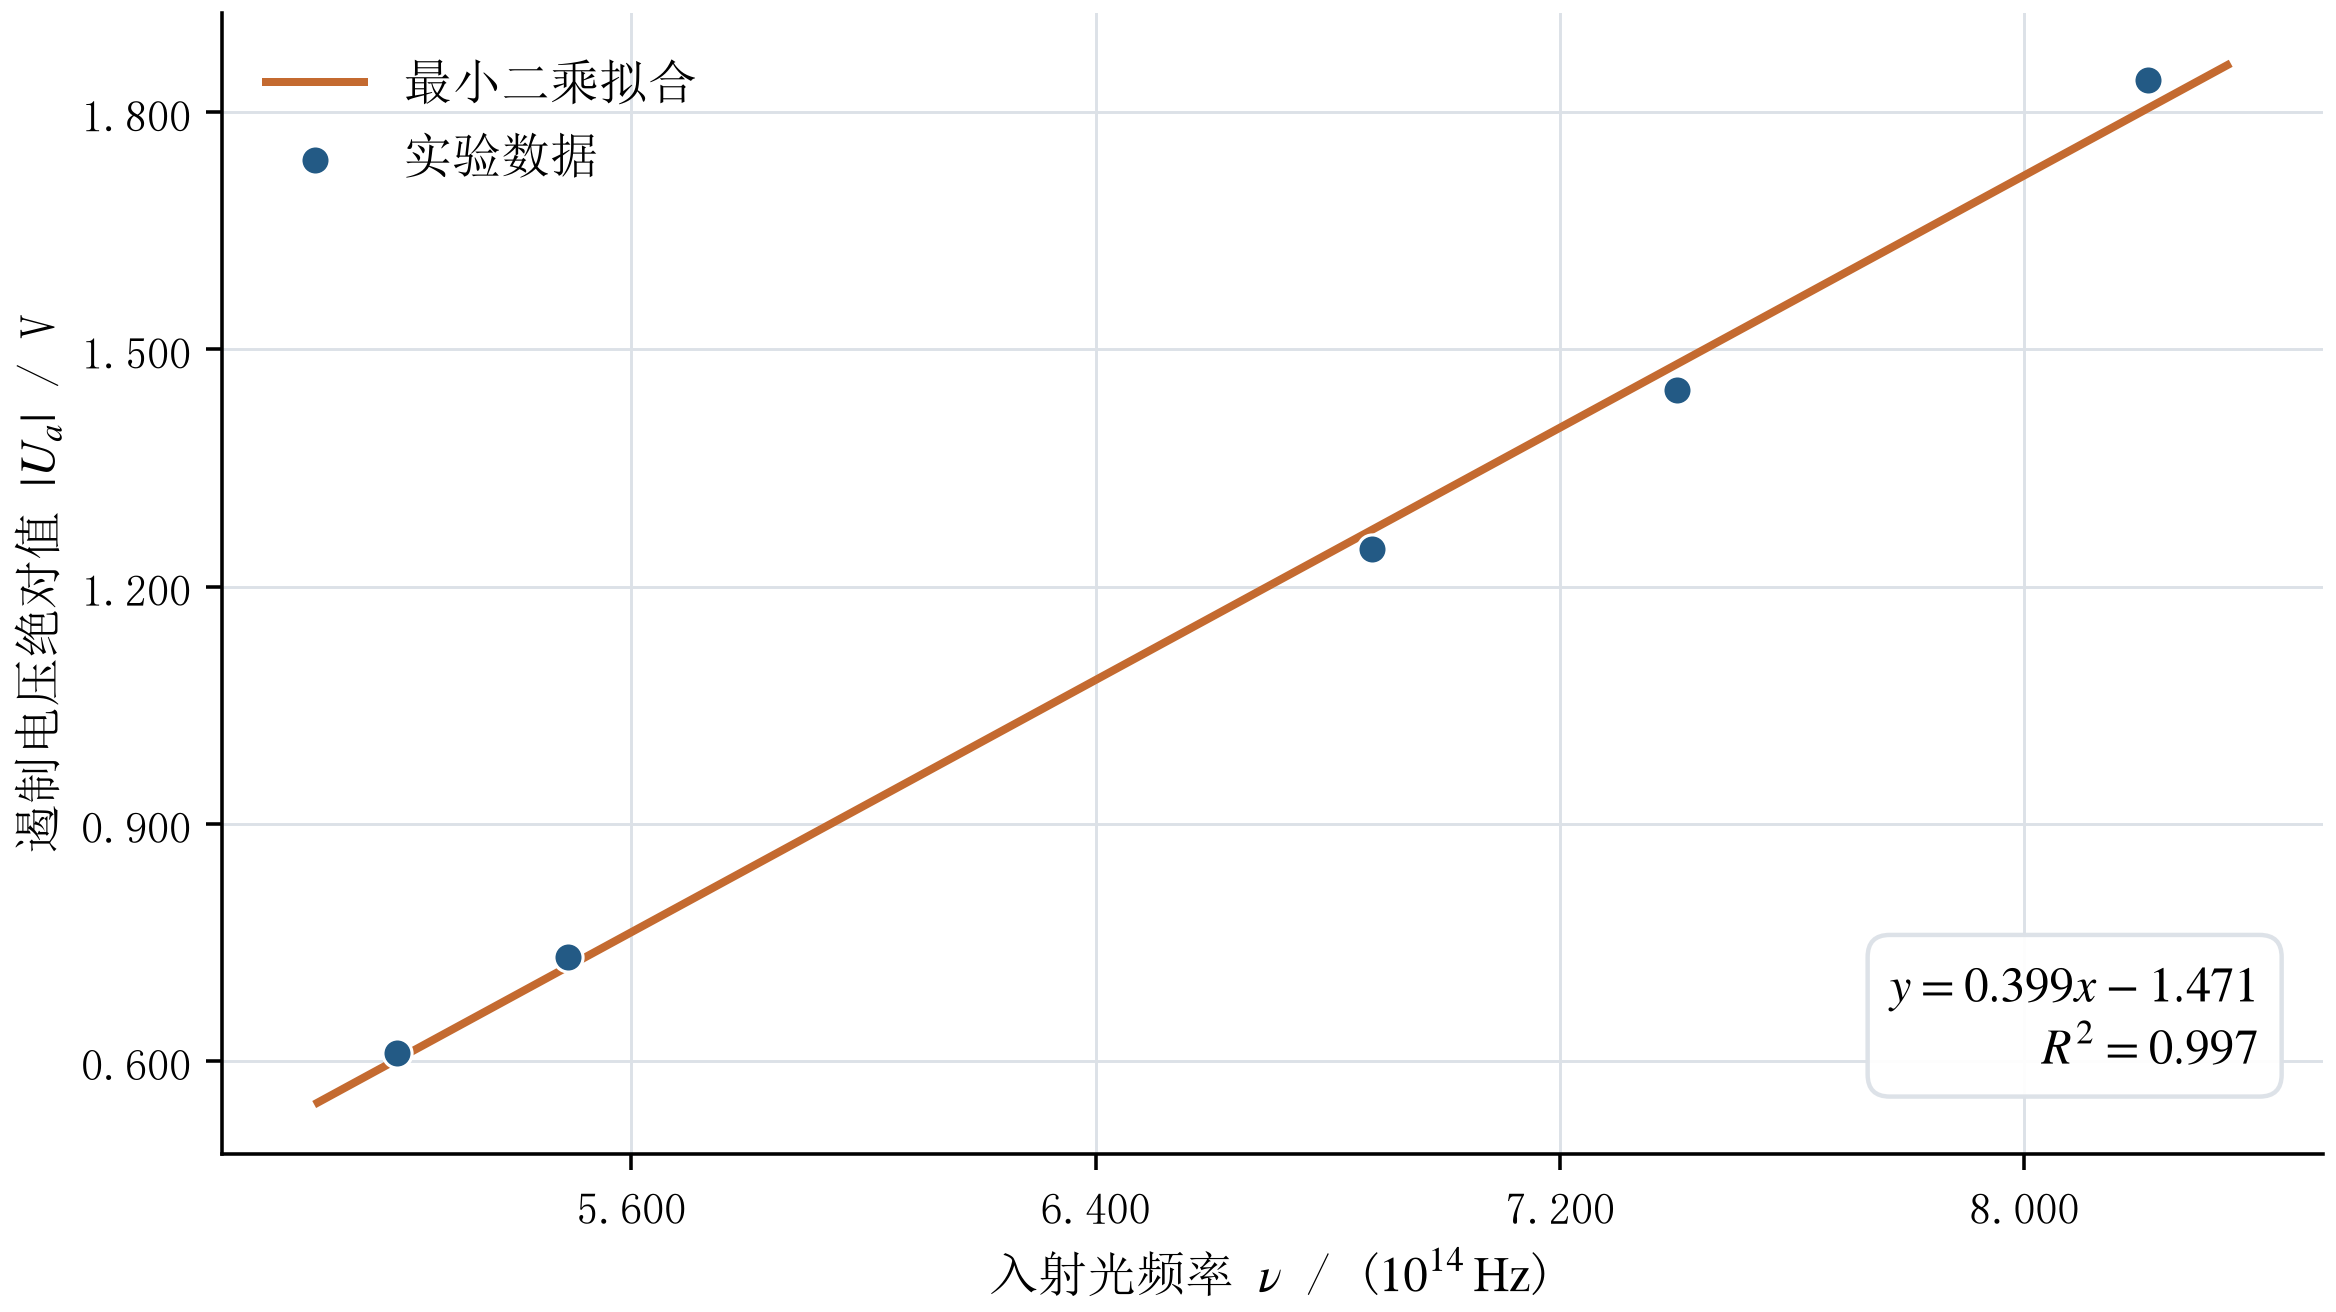
\includegraphics[width=0.6\textwidth]{figures/图6.png}
      \caption{测定普朗克常量的曲线}
    \end{figure}

    令$x=\nu/(10^{14}\,\mathrm{Hz})$，拟合得到
    \[
      \frac{U}{\mathrm{V}}=0.399x-1.471,\qquad R^2=0.997
    \]

    根据$U=(h/e)\nu-W/e$，拟合斜率为$k=3.989\times10^{-15}\,\mathrm{V\,s}$，由此得到
    \[
      h=ek=6.391\times10^{-34}\,\mathrm{J\,s}
    \]
    
    与公认值$h_0=6.626\times10^{-34}\,\mathrm{J\,s}$相比，实验结果偏小，相对误差为
    \[
      E=\frac{|h-h_0|}{h_0}\times100\%=3.555\%
    \]

    实验点近似分布在一条直线上，表明遏制电压绝对值随入射光频率增大而增大，与爱因斯坦光电效应方程相符。

    \subsubsection{不同距离和孔径下的伏安特性曲线}
    实验测定数据如下：

    \begin{table}[H]
      \centering
      \caption{伏安特性曲线（滤光片波长：$436\,\mathrm{nm}$，光阑孔径$4\,\mathrm{mm}$，光源距离$40\,\mathrm{cm}$）}
      \setlength{\tabcolsep}{5pt}
      \begin{tabular}{ccccccccccccc}
        \toprule
        光电管电压$U_{\mathrm{AK}}$（V） & -1.57 & 0.65 & 2.81 & 4.43 & 6.10 & 8.73 
        & 11.52 & 14.56 & 18.50 & 21.65 & 24.85 & 28.60 \\
        \midrule
        电流$i$（$10^{-11}\,\mathrm{A}$） & 0 & 58 & 198 & 305 & 387 & 503 & 578 & 646 & 713 & 756 & 791 & 831 \\
        \bottomrule
      \end{tabular}
    \end{table}

    \begin{table}[H]
      \centering
      \caption{伏安特性曲线（滤光片波长：$436\,\mathrm{nm}$，光阑孔径$8\,\mathrm{mm}$，光源距离$34\,\mathrm{cm}$）}
      \setlength{\tabcolsep}{5pt}
      \begin{tabular}{ccccccccccccc}
        \toprule
        光电管电压$U_{\mathrm{AK}}$（V） & -2.67 & 0.02 & 2.85 & 4.03 & 7.10 & 9.35 
        & 12.62 & 14.91 & 17.57 & 20.20 & 22.22 & 27.25 \\
        \midrule
        电流$i$（$10^{-10}\,\mathrm{A}$） & 0 & 23 & 127 & 177 & 267 & 318 & 360 & 395 & 421 & 442 & 458 & 489 \\
        \bottomrule
      \end{tabular}
    \end{table}
   
    将两组数据中的电流换算为相同单位，绘制在同一坐标系中，如图7所示。
    \begin{figure}[H]
      \centering
      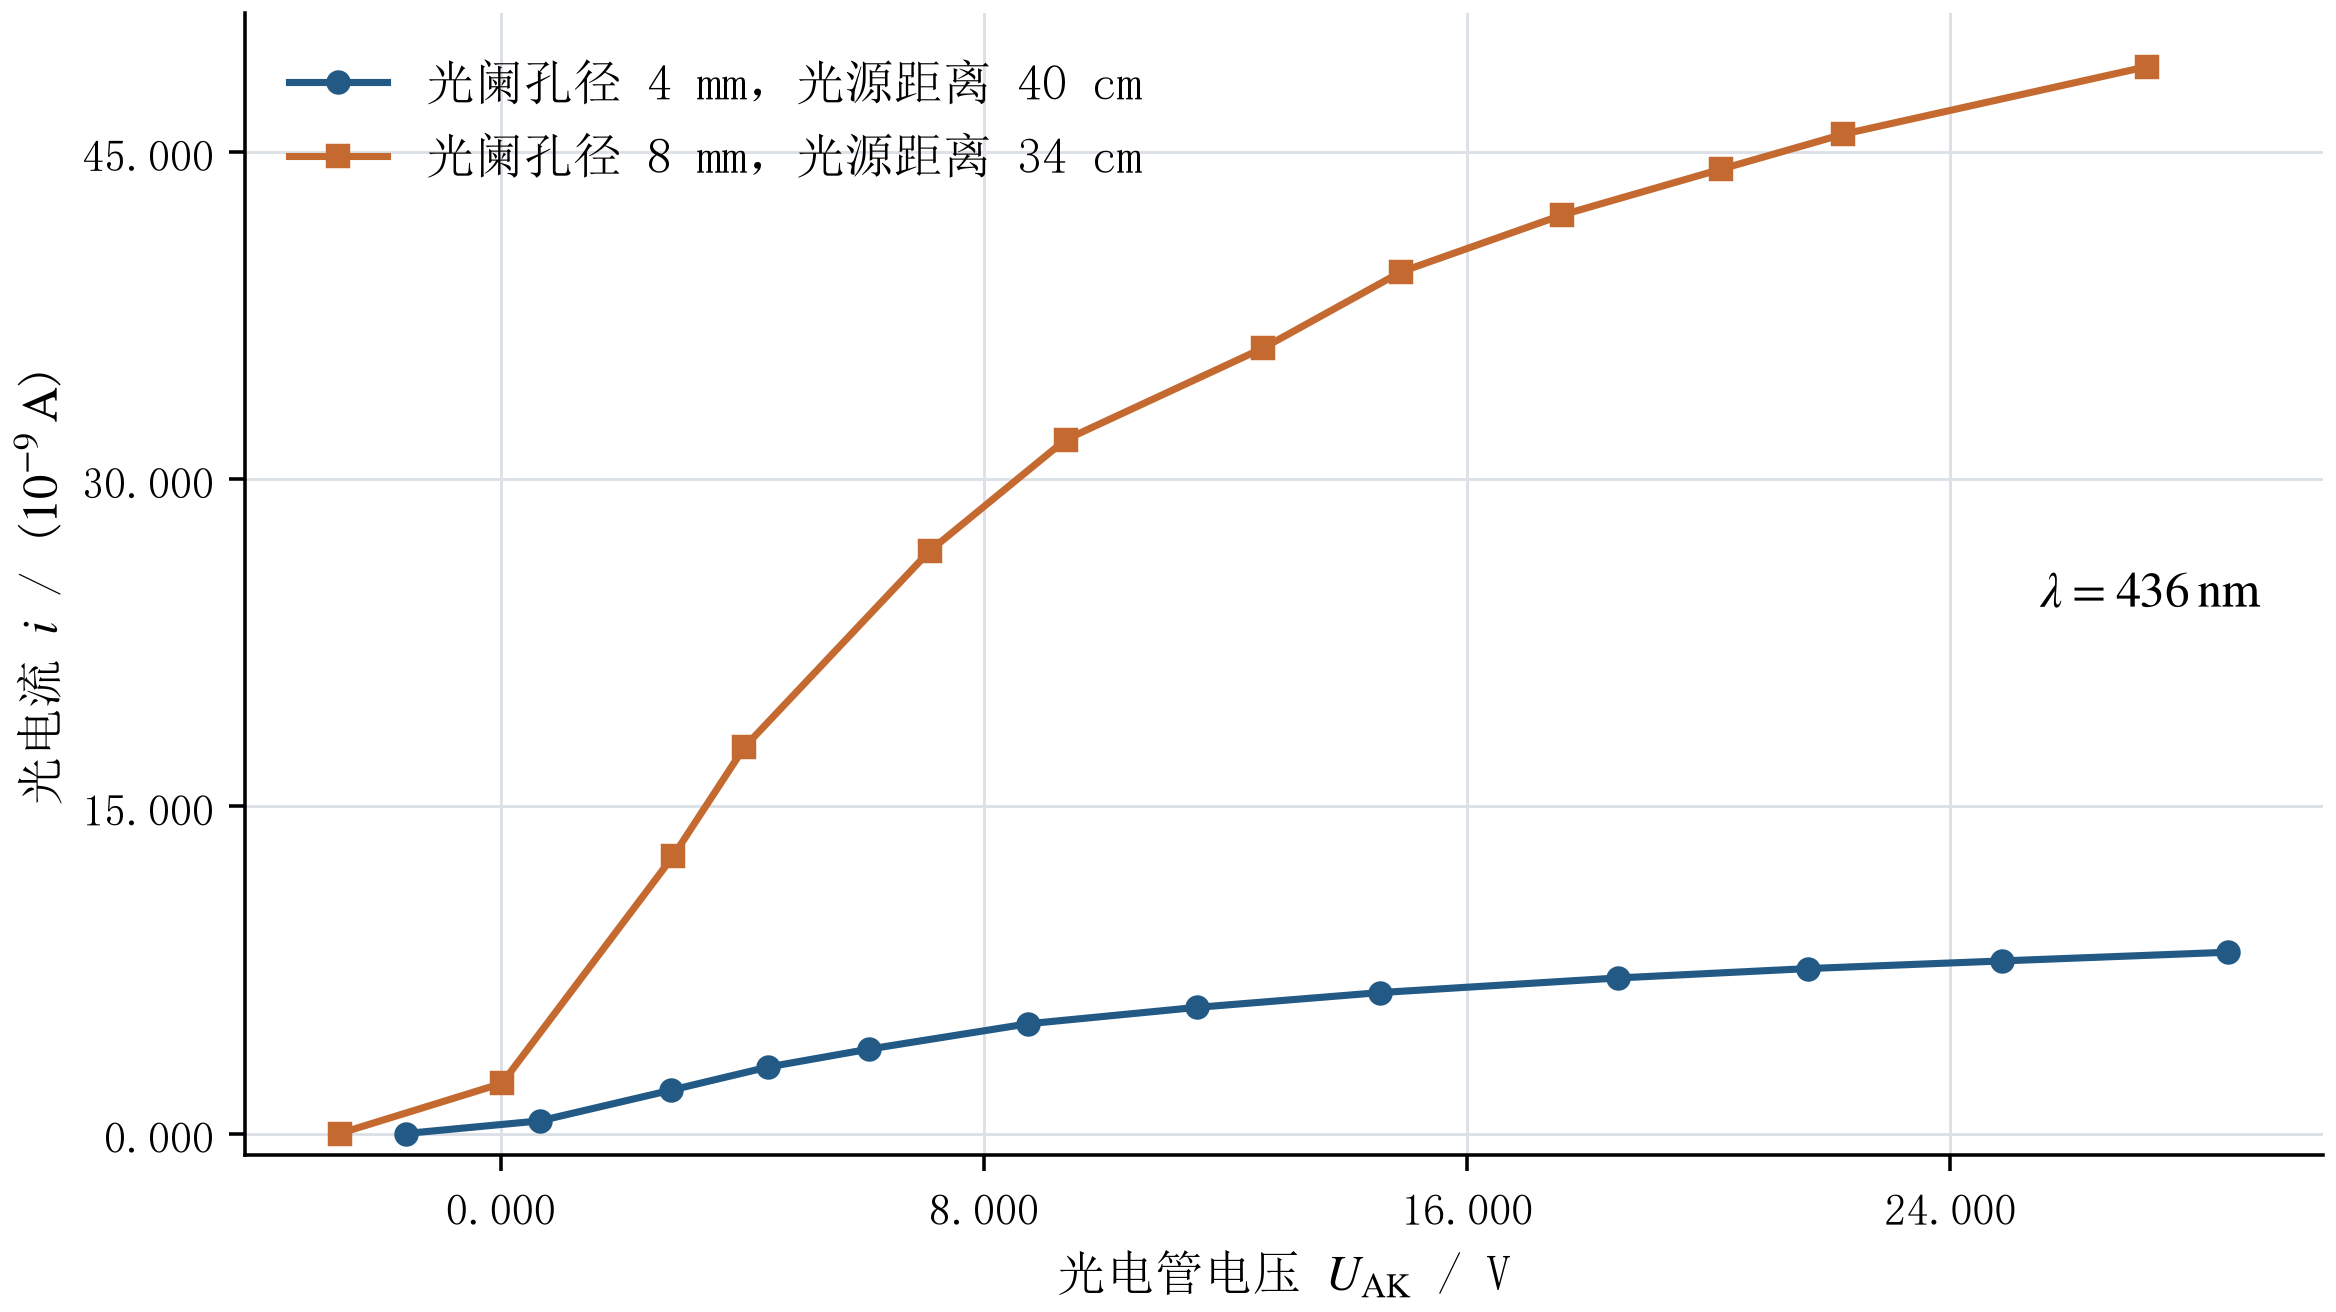
\includegraphics[width=0.6\textwidth]{figures/图7.png}
      \caption{不同光阑孔径和光源距离下的伏安特性曲线}
    \end{figure}

    随正向电压增大，阳极收集到的光电子逐渐增多，电流先较快上升，随后增速减缓。
    孔径较大、距离较近时，进入光电管的光通量更大，因此电流更大。
    两组曲线在最高测量电压处仍呈现明显上升的趋势，尚未出现稳定平台，因此本次测量未达到完全饱和但已接近饱和。

    \subsubsection{饱和光电流与距离和孔径的关系}
    实验测定数据如下：

    \begin{table}[H]
      \centering
      \caption{饱和光电流与距离的关系（光阑孔径：$4\,\mathrm{mm}$，滤光片波长：$436\,\mathrm{nm}$）}
      \begin{tabular}{cccccc}
        \toprule
        光源距离$L$（cm） & 40 & 38 & 36 & 34 & 32 \\
        $L^{-2}$（$10^{-4}\,\mathrm{cm}^{-2}$） & 6.250 & 6.925 & 7.716 & 8.651 & 9.766 \\
        \midrule
        饱和电流$i_s$（$10^{-11}\,\mathrm{A}$） & 824 & 951 & 1118 & 1290 & 1554 \\
        \bottomrule
      \end{tabular}
    \end{table}

    固定光阑孔径，以$L^{-2}$为横坐标作图，得到图8。

    \begin{figure}[H]
      \centering
      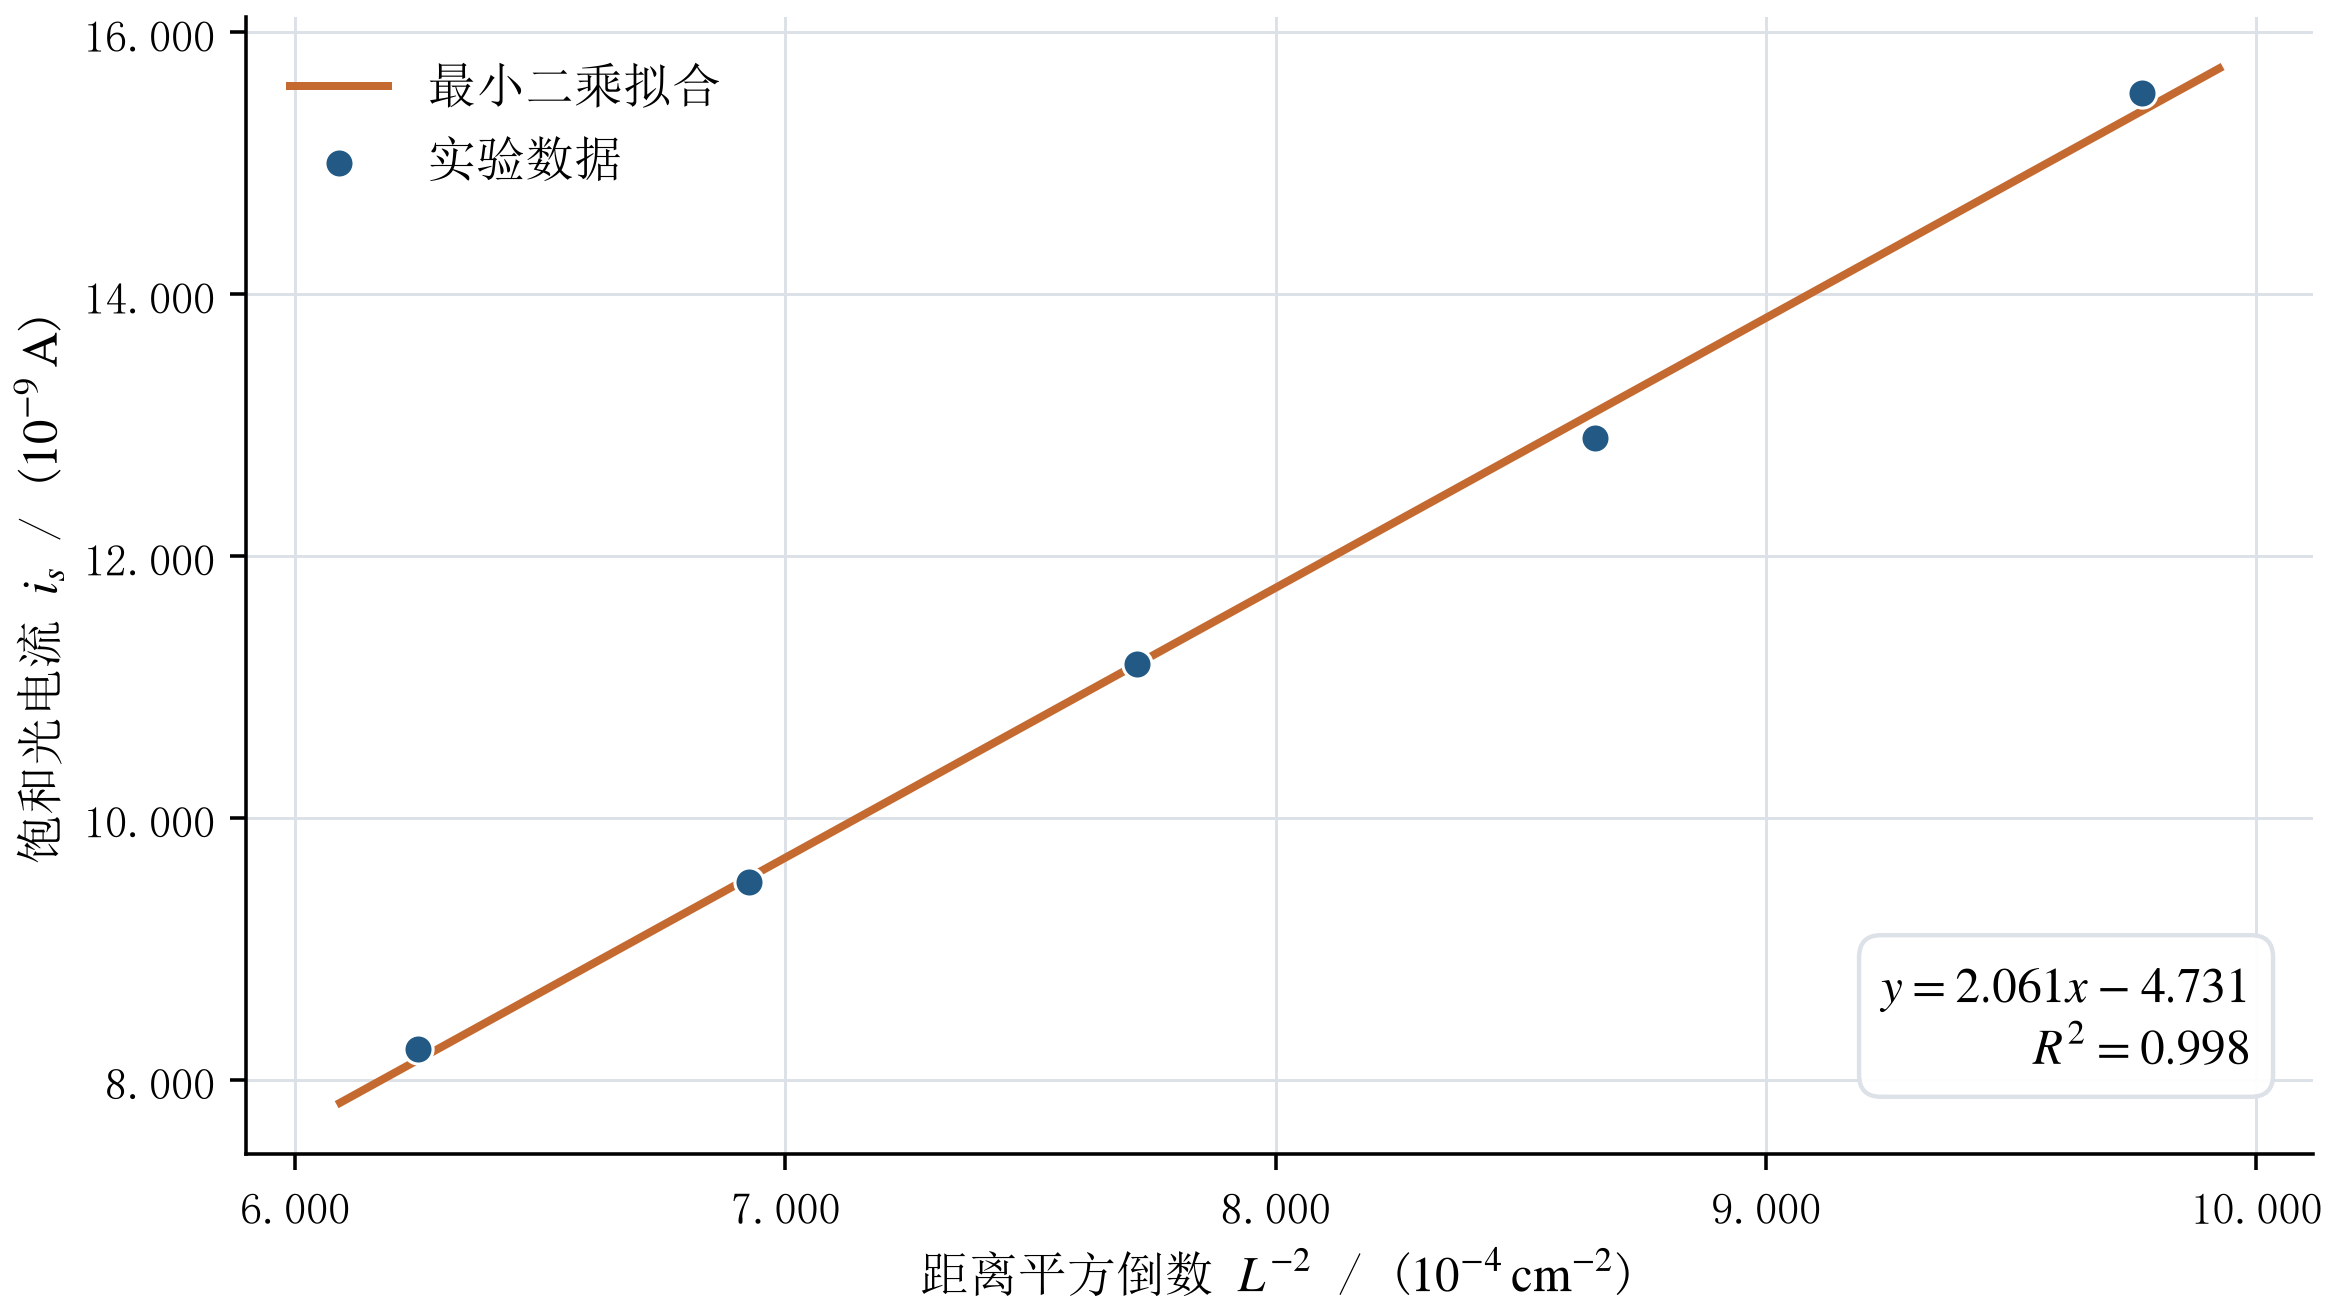
\includegraphics[width=0.6\textwidth]{figures/图8.png}
      \caption{饱和光电流与光源距离平方倒数的关系}
    \end{figure}

    线性拟合结果为
    \[
      \frac{i_s}{10^{-9}\,\mathrm{A}}
      =2.061\,\frac{L^{-2}}{10^{-4}\,\mathrm{cm}^{-2}}-4.731,
      \qquad R^2=0.998
    \]

    实验数据表明，光源距离减小时，饱和光电流增大，且与$L^{-2}$呈良好的线性关系。
    这是因为光源越近，阴极处的光照越强，单位时间内逸出的光电子越多，因此饱和光电流越大。

    \begin{table}[H]
      \centering
      \caption{饱和光电流与孔径的关系（光源距离：$40\,\mathrm{cm}$，滤光片波长：$436\,\mathrm{nm}$）}
      \begin{tabular}{cccc}
        \toprule
        光阑孔径$\Phi$（mm） & 2 & 4 & 8 \\
        $\Phi^2$（$\mathrm{mm}^2$） & 4.000 & 16.000 & 64.000 \\
        \midrule
        饱和电流$i_s$（$10^{-10}\,\mathrm{A}$） & 21.7 & 84.2 & 336.0 \\
        \bottomrule
      \end{tabular}
    \end{table}

    固定光源距离，以光阑孔径平方$\Phi^2$为横坐标作图，得到图9。

    \begin{figure}[H]
      \centering
      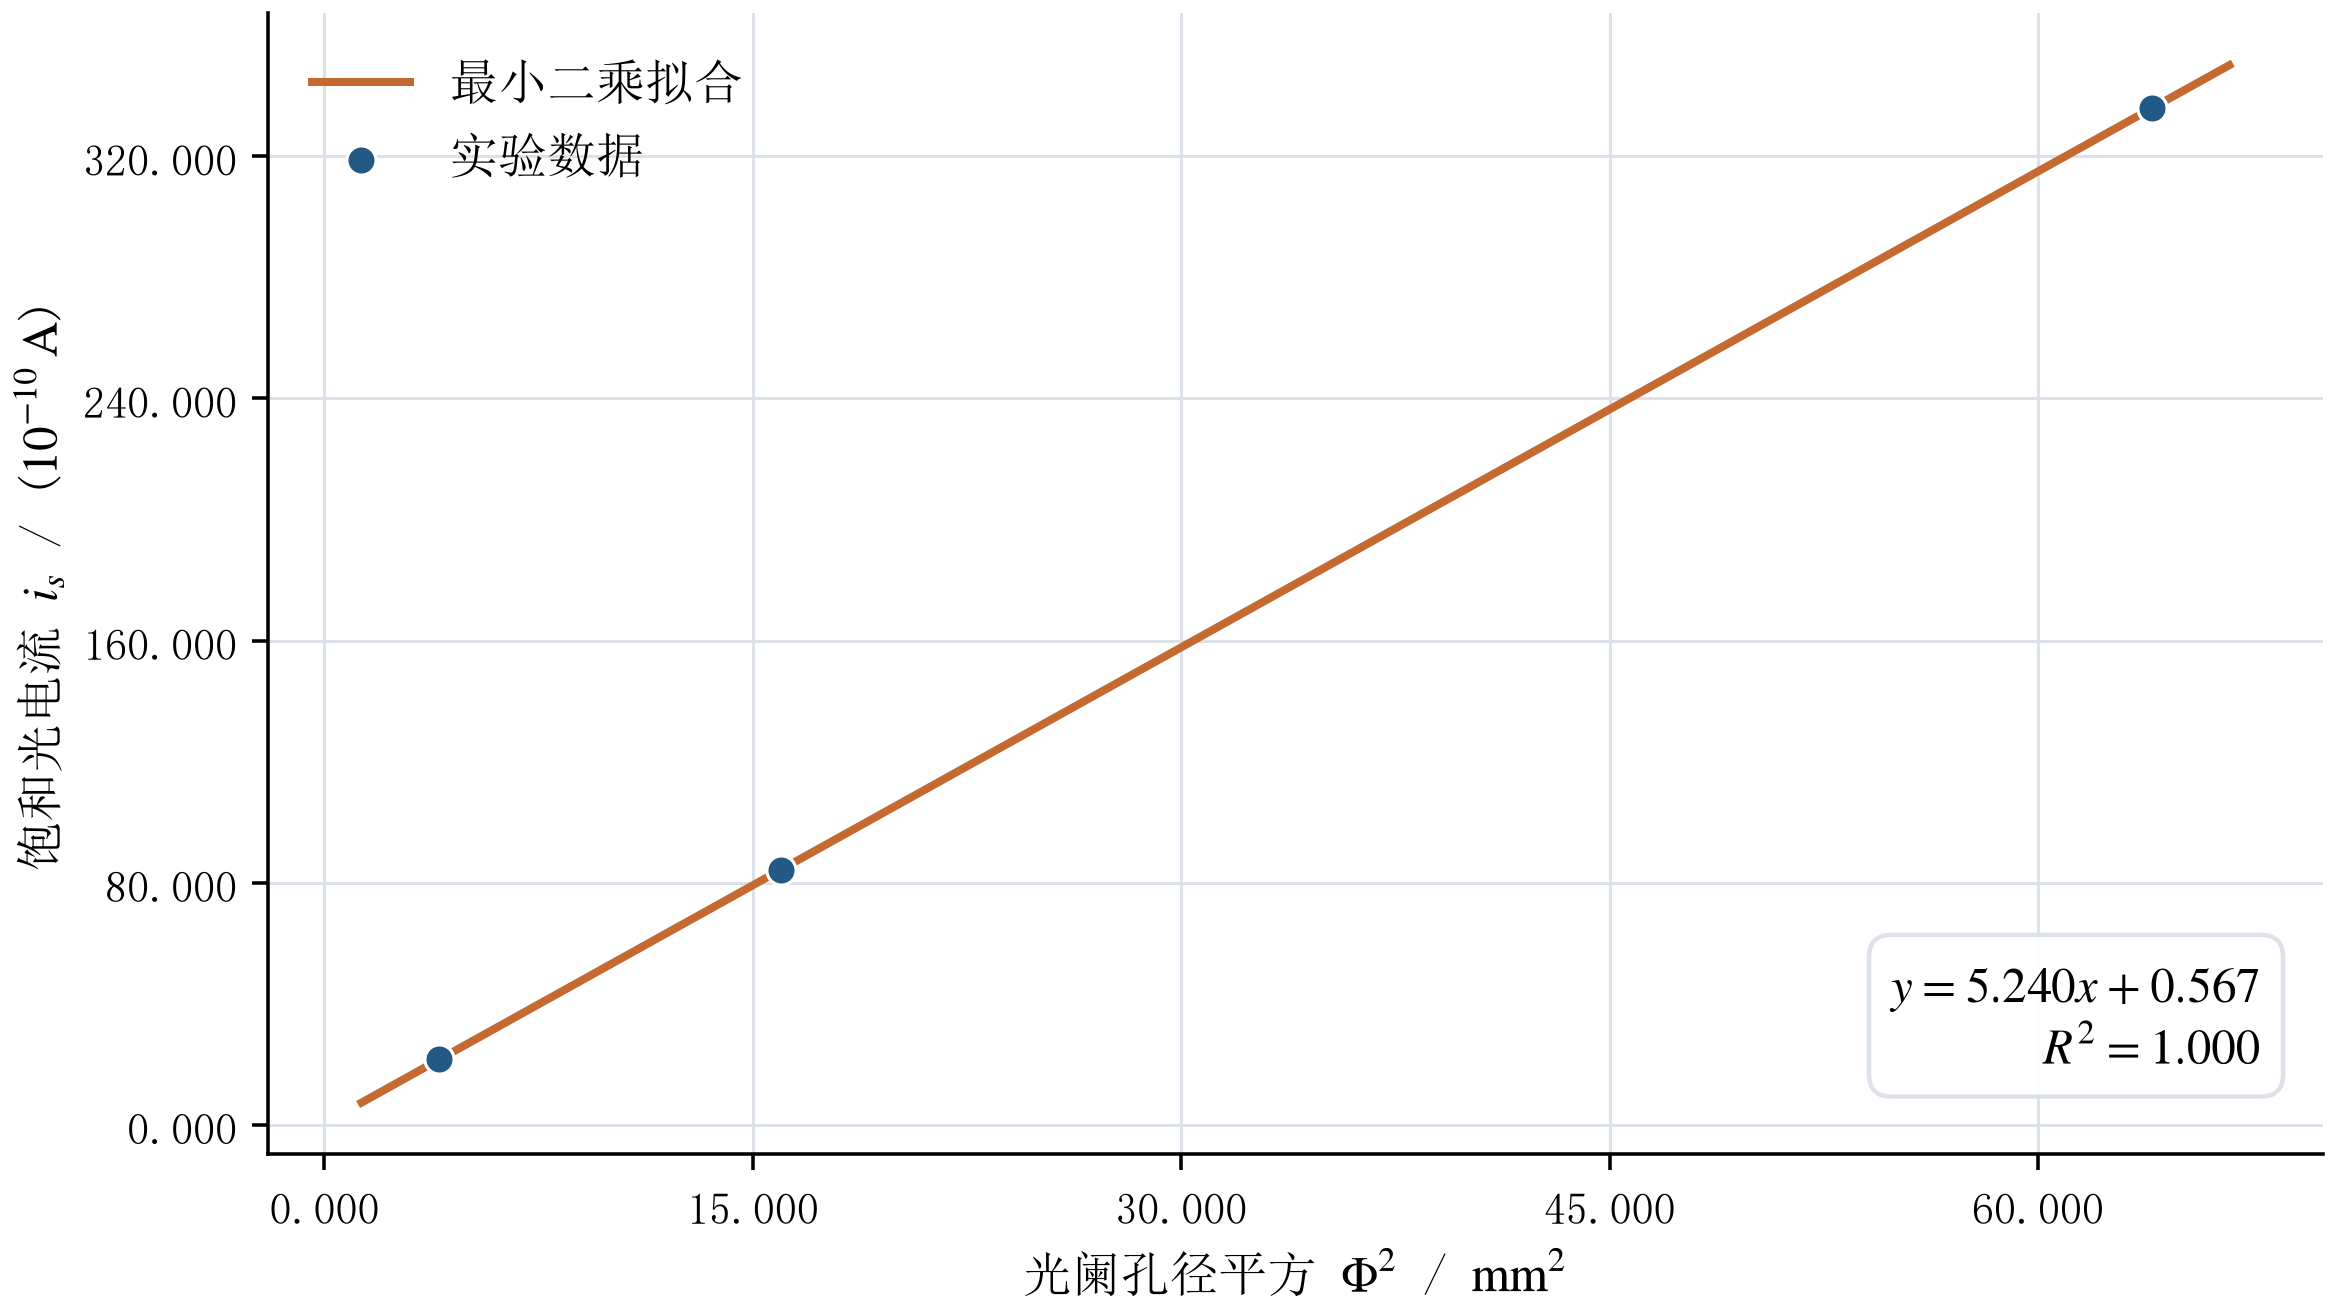
\includegraphics[width=0.6\textwidth]{figures/图9.png}
      \caption{饱和光电流与光阑孔径平方的关系}
    \end{figure}

    线性拟合结果为
    \[
      \frac{i_s}{10^{-10}\,\mathrm{A}}
      =5.240\,\frac{\Phi^2}{\mathrm{mm}^2}+0.567,
      \qquad R^2=1.000
    \]

    实验数据表明，饱和光电流随光阑孔径增大而增大，并与孔径平方$\Phi^2$近似成正比。
    这是因为光阑通光面积与$\Phi^2$成正比，增大孔径使入射光子数增多，单位时间内逸出的光电子随之增加，从而使饱和光电流增大。

  \subsection{误差分析（10分）}
  \begin{enumerate}
    \item 仪器调零与读数：零点漂移、电流读数波动和电压调节精度影响零电流位置的判断，进而影响遏制电压及拟合斜率。
    \item 光源与滤光片：汞灯亮度波动、杂散光及滤光片的有限带宽，使实际光强与入射光频率存在偏差。
    \item 距离与光路：距离读数、测量基准及光阑对准偏差影响阴极实际接收的光照强度。
    \item 饱和电压选取：正向电压不足时，光电子未被完全收集，使测得的电流低于饱和值。
  \end{enumerate}

\section{实验探讨与思考题（10分）}

  \subsection{实验探讨}
  通过实验，我认识到光电效应体现了光的粒子性，并加深了对光电流影响因素的认识。
  只有光子能量足以克服逸出功，电子才能逸出；入射光频率越高，光电子最大初动能越大，截止电压绝对值也越大。
  同一频率下，增强光照主要增加逸出电子数，使饱和光电流增大。
  当阳极几乎收集全部光电子时，继续升高正向电压，电流基本不再增加。
  因此，频率决定电子最大初动能，光强影响光电子的发射数量。

  \subsection{思考题}

    \subsubsection{测定普朗克常量的关键是什么？怎样根据光电管的特性曲线选取适宜的测定遏制电压\texorpdfstring{$U_a$}{Uₐ}的方法？}
    测定普朗克常量的关键是准确测出不同频率单色光对应的遏制电压，并由$U_a$--$\nu$直线的斜率求得$h$。
    取$U_a=|U_{AK}|$，若拟合式为$U_a=k\nu+b$，则$h=ek$。

    测量方法应根据伏安特性选择：正向电流上升快、反向电流及暗电流很小时，可取光照与暗电流曲线交点对应的电压，即交点法；
    暗电流可忽略时，近似采用零电流法。
    若反向电流较大但很快饱和，则宜取反向电流开始饱和处的拐点电压，即拐点法。
    本实验所用仪器的反向电流与暗电流较小，故采用零电流法测量遏制电压。

    \subsubsection{从遏制电压\texorpdfstring{$U_a$}{Uₐ}与入射光的频率\texorpdfstring{$\nu$}{ν}的关系曲线中，你能确定阴极材料的逸出功吗？}
    由爱因斯坦光电效应方程
    \[
      U_a=\frac{h}{e}\nu-\frac{W}{e}=k\nu+b
    \]
    可知，若以遏制电压的绝对值作图，纵轴截距为$b=-W/e$，因此逸出功$W=-eb$；
    也可由横轴截距求出极限频率$\nu_0$，再由$W=h\nu_0$计算。
    
    \subsubsection{本实验存在哪些误差来源？实验中如何解决这些问题？}
    误差来源见3.2误差分析，主要与仪器调零和读数、光源与滤光片、距离与光路、饱和电压选取有关。

    为解决这些问题，可以这样做。
    实验时应充分预热仪器和汞灯，换挡后重新调零；在零电流附近细调电压并重复测量；
    正确选用滤光片并遮挡杂散光，保持光路对准，统一距离测量基准；
    测量饱和光电流时逐步提高正向电压，待电流进入稳定平台后再读数。
    
\vspace*{\fill} % 使下面内容在页面底部显示
\noindent
\begin{minipage}{\textwidth}
  注意事项：

  \begingroup
    \setlength{\leftskip}{2em} % 1--4整体向右缩进两个汉字宽度
    1. 用PDF格式上传“实验报告”，文件名：学生姓名+学号+实验名称+周次。

    2. “实验报告”必须递交在“学在浙大”本课程内对应实验项目的“作业”模块内。

    3. “实验报告”成绩必须在“浙江大学物理实验教学中心网站”-“选课系统”内查询。

    4. 教学评价必须在“浙江大学物理实验教学中心网站”-“选课系统”内进行，学生必须进行教学评价，才能看到实验报告成绩，教学评价须在本次实验结束之后3天内进行。\par
  \endgroup

  \begin{center}
    {\CJKfontspec[AutoFakeBold=2.5]{SimSun}\bfseries 浙江大学物理实验教学中心制}
  \end{center}
\end{minipage}

\end{document}
